\documentclass{article}

% if you need to pass options to natbib, use, e.g.:
% \PassOptionsToPackage{numbers, compress}{natbib}
% before loading nips_2016
%
% to avoid loading the natbib package, add option nonatbib:
% \usepackage[nonatbib]{nips_2016}

\usepackage{nips_2016}

% to compile a camera-ready version, add the [final] option, e.g.:
% \usepackage[final]{nips_2016}

\usepackage[utf8]{inputenc} % allow utf-8 input
\usepackage[T1]{fontenc}    % use 8-bit T1 fonts
\usepackage{hyperref}       % hyperlinks
\usepackage{url}            % simple URL typesetting
\usepackage{booktabs}       % professional-quality tables
\usepackage{amsfonts}       % blackboard math symbols
\usepackage{nicefrac}       % compact symbols for 1/2, etc.
\usepackage{microtype}      % microtypography
\usepackage[final]{graphicx}


\title{Accuracy of secondary protein structure prediction tools for chromoproteins and fluorescent proteins}

\begin{document}
% \nipsfinalcopy is no longer used

 Rachael C.~Kretsch \\
 Mathematics of Big Data, Fall 2016\\
 Harvey Mudd College\\
 \texttt{rkretsch@g.hmc.edu} \\

\maketitle

\begin{abstract}
   abstract...
\end{abstract}

\section{Introduction}

\subsection{Secondary protein structure prediction}

This project aims to look at methods to predict secondary protein structure. Protein structure prediction is a major field of study and is a problem that takes massive computational power to solve. There are two main approaches looking from a biochemical point of view. The first is isolated the protein, crystallizing it, and performing crystal chromatography to figure out the structure. This structure is relaxed into its hypothesized structure via molecular dynamics. I have previously done work on molecular dynamic methods, but now I would like to look at it from the other direction. One of the most plentiful and easy to obtain biological data is DNA sequence. From the DNA sequence of a coding region there are simply rules to propose a great starting point for the protein's amino acid sequence. The problem of predicting the 3D structure from an amino acid sequence is extremely hard. I will reduce this problem to simpler features. My aim is to look at how we can use the amino acid sequence, the primary structure, to deduce secondary structure components like beta sheets, alpha helices, and coils. 

\subsection{Fluorescent proteins and chromoproteins}
\section{Methods and materials}

\subsection{Logistic regression method implementation}

\subsection{Literature method testing}

\subsubsection{GORIV}

\subsubsection{SOPM}

\subsubsection{s2D}


\section{Results}

\subsection{Logistic regression}

\begin{figure}[h]
  \centering
  \fbox{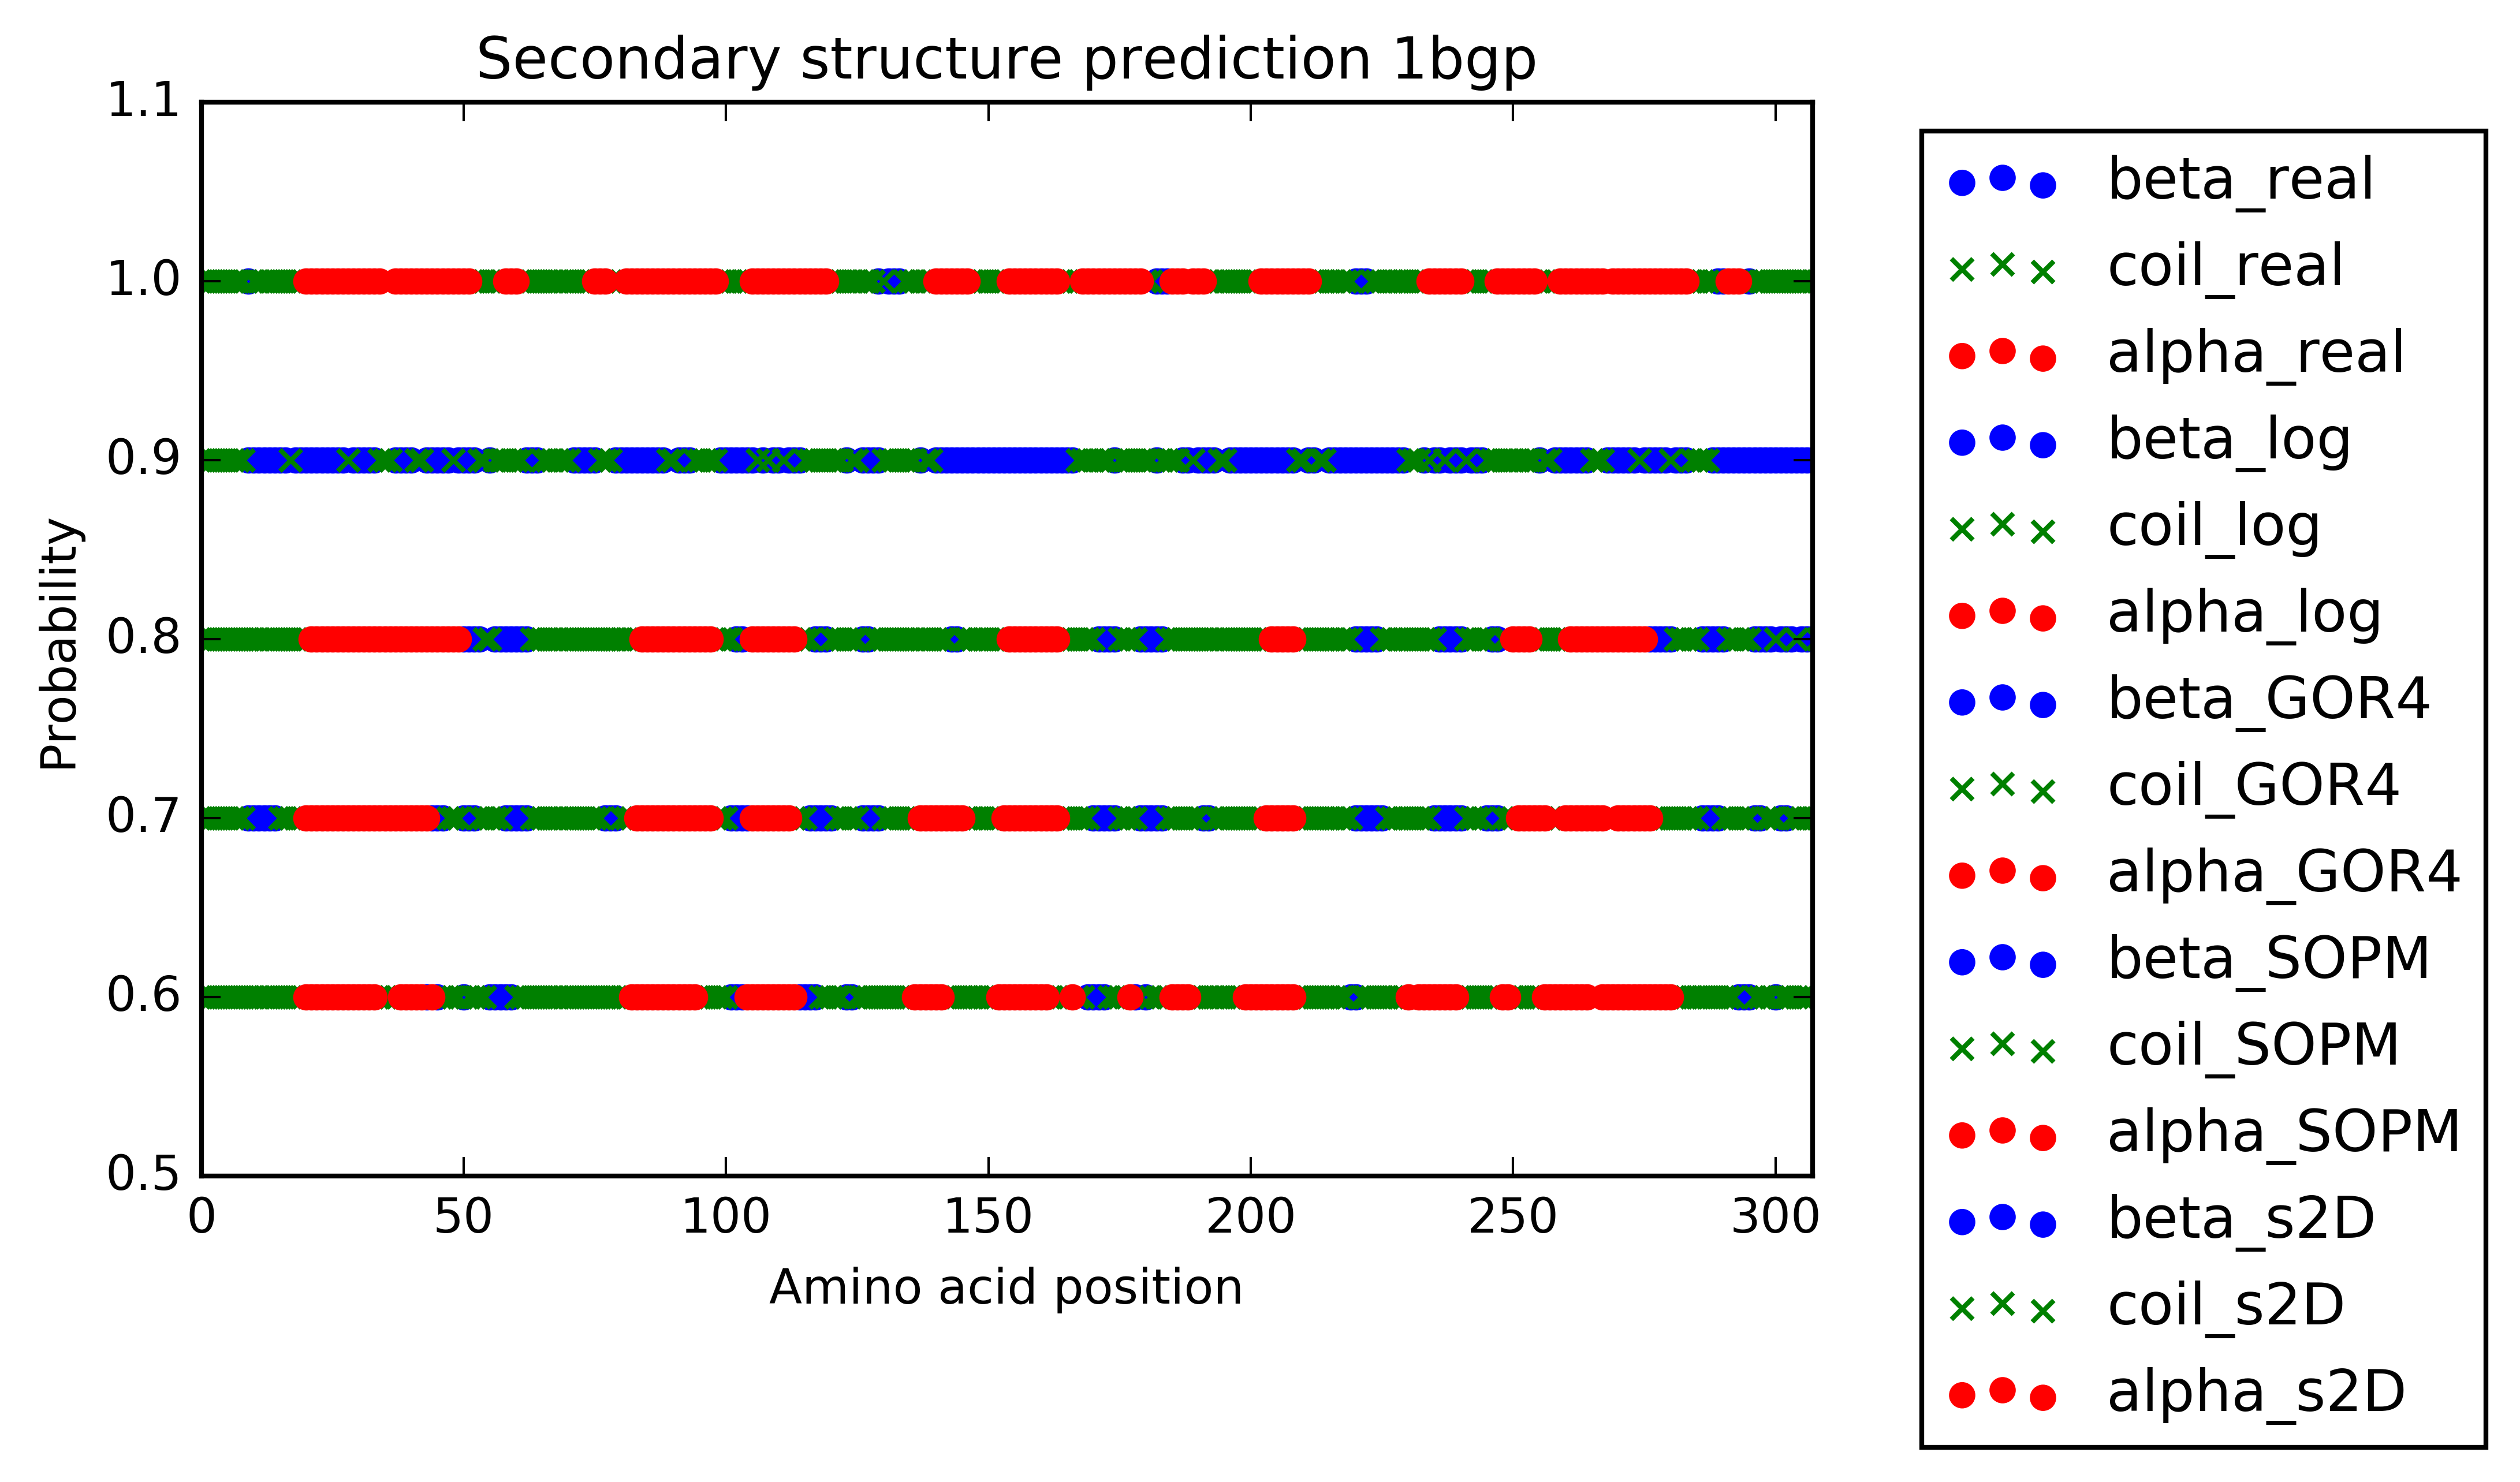
\includegraphics[width=\textwidth]{1bgp.png}}
  \caption{Sample figure caption.}
\end{figure}

\begin{figure}[h]
  \centering
  \fbox{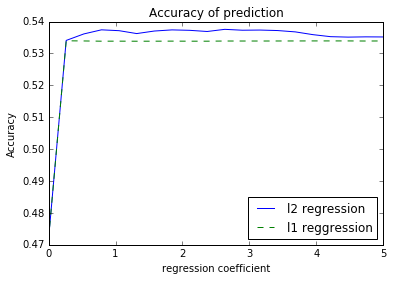
\includegraphics[width=\textwidth]{reg_values}}
  \caption{Sample figure caption.}
\end{figure}



\subsection{Method comparison}


\begin{table}[t]
  \caption{Accuracy of various secondary structure prediction methods}
  \centering
  \begin{tabular}{lll}
    \toprule
    Method     & Accuracy on data set (\%)    & Reported accuracy (\%)\\
    \midrule
    Logistic regression & 54 & -     \\
    GORIV     & 48 & 64      \\
    SOPM     & 51      & 69  \\
    s2D     & 64       & 85-88  \\
    \bottomrule
  \end{tabular}
\end{table}

\begin{table}[t]
  \caption{Accuracy of methods for specific proteins}
  \centering
  \begin{tabular}{lllll}
    \toprule
    \multicolumn{5}{c}{Accuracies (\%)}\\
    \cmidrule{2-5}
    Protein ID & Logistic regression & GORIV & SOPM & s2D\\
    \midrule
    1bgp & 25 & 64&62&64 \\
    4q7t & 25 & 44 & 42 & 67 \\
    4qgw & 25 & 69 & 61 & 83 \\
    5h88 & 26 & 37&37&57 \\
    4l1s & 26 & 64&52&70 \\
    
    5h89 & 27 & 37&39&60 \\
    3s0f & 27 & 49 & 58 & 70 \\
    4q9w & 27 & 51&55&70 \\
    3rwt & 27 & 37&35&48 \\
    5hzo & 28 & 37 & 46 & 64 \\
    \midrule
    1bfp & 60 & 48&60&77 \\
    3ekh & 60 & 54&61&55 \\
    3ned & 60 & 40&46&73 \\
    4k3g & 60 & 49&54&59 \\
    3cfc & 60 & 58 &60&61 \\
    
    1xkh & 60 & 50&48&47 \\
    2wht & 60 & 37&58&70 \\
    4w6b & 60 & 44&54&69 \\
    4xvp & 60 & 44&49&52 \\
    3dqh & 60 & 42&56&73 \\
    \bottomrule
  \end{tabular}
\end{table}

\section{Discussion}

An interesting future problem could be to implement a machine learning algorithm to address post-transcriptional modifications. 


\subsubsection*{Availability}

All data, source code, and text from this project can be found at this git hub repo: \url{https://github.com/hmc-cs-rkretsch/Secondary-Protein-Structure}

\subsubsection*{Acknowledgments}

I would like to thank Professor Gu for teaching me the basics that allowed me to better understand these complex and cool methods. Thank you to all the graders for making this course reliable. And finally, thank you to my past research advisors and professors for helping me find my areas of interests.

\section*{References}

\small

[1] Touw, W.G.\ \& Baakman, C.\ \& Black, B. \ \& te Beek, T.AH.\ \& Kreiger, E.\ \& Joosten, R.P.\ \&
Vriend, G.\ (2015) A series of PBD related databases for everyday needs.
for connectionist rule extraction.  {\it Nucleic Acids Research}, 43(Database issue): D364-D368.

[2] Kabsch W.\ \& Sander C.\ (1983) Dictionary of protein secondary structure: pattern recognition of hydrogen-bonded and geometrical features {\it Biopolymers}, 983 22 2577-2637. PMID: 6667333; UI: 84128824.

[3] Cambria, A.\ (2009) Hidropathy Clustering Assisted Methods. http://www.acbrc.org/hcam.html

[4] Garnier, J.\ \& Gibrat, J.F.\ \& Robson, B.\ (1996) GOR Method for Predicting Protein Secondary Structure from Amino Acid Sequence. {\it Method in Enzymology}. 266:540-53.

[5] Geourjon C.\ \& Deleage G.\ (1994) SOPM: a self-optimimization mehtod for protein secondary structure prediction. {\it Protein Engineering.} 7(2):157-64.

[6] Karypis, G.\ (2006) YASSPP: Better Kernels and Coding Schemes Lead to Improvements in Protein Secondary Structure Prediction. {\it Proteins.} 64:575-86.

[7] Singh, M.\ (2001) Predicting Protein Secondary and Supersecondary Structure. Princeton University. CRC Press.

[8] Sormanni, P.\ \& Camilloni, C.\ \& Fariselli, P.\ \& Vendruscolo, M.\ (2015) The s2D Method: Simultaneous Sequence-Based Prediction of the Statistical Populations of Ordered and Disordered Regions in Proteins. {\it J. Mol. Biol.} 427: 982-96.

[9] Sen, T.Z.\ \& Jernigan, R.L.\ \& Garnier, J.\ \& Kloczkowski, A.\ (2005) GOR V server for protein secondary structure prediction. {\it Bioinformatics} Jun 1; 21(11): 2787?2788.

[10] RCSB Protein Data Bank. An Information Portal to 124928 Biological Structures. 739 proteins used, please see additional resources for these proteins and acknowledgments to all the scientists to whom these 739 proteins structures are acknowledged.

\end{document}
